\documentclass[9pt,journal,compsoc]{IEEEtran}
\ifCLASSOPTIONcompsoc
  \usepackage[nocompress]{cite}
\else
  \usepackage{cite}
\fi
\ifCLASSINFOpdf
\else
\fi
\hyphenation{op-tical net-works semi-conduc-tor}
\usepackage{cite}
\usepackage{amsmath,amssymb,amsfonts}
\usepackage{algorithmic}
\usepackage{graphicx}
\usepackage{textcomp}
\usepackage{xcolor}
\usepackage{graphicx}
\usepackage{subfigure}
\usepackage{CJK}
\usepackage{indentfirst}
\usepackage{amsmath}
\usepackage{upgreek}
\usepackage{tabu}
\usepackage{booktabs}
\usepackage{threeparttable}
\usepackage{tabularx}
\usepackage{multirow}
\usepackage{multicol}
\usepackage{arydshln}
\usepackage{makecell}

\begin{document}

\title{A High-Performance Design of Generalized Pipeline Cellular Array}

\author{
        Zhufei~Chu,~\IEEEmembership{Member,~IEEE,}
        Huiming~Tian,
        Zeqiang~Li,
        Yinshui~Xia,
        and Lunyao~Wang
        % <-this % stops a space
\thanks{
(\emph{Corresponding author}: \emph{Zhufei Chu}).
Z. Chu, H. Tian, Z. Li, Y. Xia, and L. Wang are with the Faculty of Electrical Engineering and Computer Science, Ningbo
University, Ningbo 315211, China. (email:chuzhufei@nbu.edu.cn)
}}

%\author{TBD}

%\author{Zhufei Chu,~\IEEEmembership{Member}, Huiming Tian, Lunyao Wang and Yinshui Xia\IEEEcompsocthanksitem J. Doe and J. Doe are with Anonymous University.s}
%       ~\IEEEmembership{}
%        ~\IEEEmembership{}
%\IEEEcompsocitemizethanks{\IEEEcompsocthanksitem M. Shell was with the Department
%of Electrical and Computer Engineering, Georgia Institute of Technology, Atlanta,
%GA, 30332.\protect\\
%E-mail: see http://www.michaelshell.org/contact.html
%\IEEEcompsocthanksitem J. Doe and J. Doe are with Anonymous University.}% <-this % stops an unwanted space
%\thanks{Manuscript received April 19, 2005; revised August 26, 2015.}}




\markboth{IEEE Computer Architecture Letters}%
{Chu \MakeLowercase{\textit{et al.}}: A High-Performance Design of Generalized Pipeline Cellular Array}

\IEEEtitleabstractindextext{%
\begin{abstract}
In this letter, we proposed a high-performance quantum-dot cellular automata (QCA) design of generalized pipeline cellular array (GPCA). The GPCA can perform all the basic arithmetic operations using only one arithmetic cell. Due to its flexibility, the high-performance GPCA design is of high interest for large-scale QCA designs.
We proposed both the arithmetic unit and control unit designs of GPCA using a hybrid logic network that represented by majority-of-three (MAJ), inverter (NOT), and three-input exclusive-OR (XOR$_3$). The introduction of XOR$_3$ operation can significantly reduce the number of gates, levels, and wire-crossings, which in turn results in less area and fewer clock cycles of QCA layout.  
On average, the proposed design can reduce the area and latency by 39.27\% and 35.89\% compared with the-state-of-art, respectively. \vspace{-2ex}
\end{abstract}

% Note that keywords are not normally used for peerreview papers.
\begin{IEEEkeywords}
majority, three-input XOR, pipeline cellular array, quantum-dot cellular automata (QCA)\vspace{-1ex}
\end{IEEEkeywords}} 


% make the title area
%\vspace{-2ex}
\maketitle
\IEEEdisplaynontitleabstractindextext
\IEEEpeerreviewmaketitle
\IEEEraisesectionheading{\section{Introduction}\label{sec:introduction}}%\vspace{-2ex}
\IEEEPARstart{H}{igh-speed} cellular array designs for arithmetic operations have attracted considerable interest for computer architecture.
The cellular array usually consists of identical arithmetic cells or units connected in an iterative array pattern.
With the transistor feature size continuing to scale down, the cellular array is becoming increasingly important.
Due to their versatility and flexibility, the arrays are suitable for large-scale integration as well as pipelining and parallel processing~\cite{agrawal1979high,majithia1976some}.   
Generalized pipeline cellular array (GPCA) is one of such array~\cite{4}, which can perform all the basic arithmetic operations in a pipeline manner. 
%There are several studies presented to address the cellular array designs, in the perspective of both high-speed arithmetic architecture design and the completeness of supported arithmetic operations~\cite{agrawal1979high,rosenfeld1983parallel,majithia1976some}.

Logic-gate implementation of the arithmetic cell has a significant impact on the performance of the cellular array.
Since complementary metal-oxide-semiconductor (CMOS) technology is gradually reaching its physical limitation in recent years, new nanotechnology circuit (e.g., quantum-dot cellular automata (QCA)~\cite{1}) and new device (e.g., two-dimensional polarity-controllable transistors~\cite{resta2018doping}) are emerging. 
These new computing paradigm demonstrated promising advantages of power consumption and device density. However, different from the conventional Boolean logic used in CMOS, the primitives of these technologies are based on majority-of-three (MAJ) logic. 

The MAJ gate over three Boolean variables $a$, $b$, and $c$ can be represented as $\mathbb{M}(a,b,c)=ab+ac+bc$.
For the three-input XOR gate (XOR$_3$), it can be also represented as the MAJ forms.  
\begin{equation}\label{equ_xor3}
\mathbb{X}(a,b,c)=a \oplus b \oplus c= \mathbb{M}(\bar a, \mathbb{M}(a,b,\bar c), \mathbb{M}(a,\bar b, c))
\end{equation} 
By setting any one of the three inputs to constant, we can obtain AND/OR/XOR operations over the remaining non-constant inputs.
As an example, $ab=\mathbb{M}(a,b,0)$ and $a\oplus b = \mathbb{X}(a,b,0)$. 

The Boolean expressions and computing architecture of $n$-bit GPCA were displayed in the 1970s~\cite{4}.
In terms of new hardware implementation, a QCA design based on the MAJ logic network for GPCA is proposed~\cite{2}.
Although the implementations of various arithmetic circuits in QCA have been investigated in the literature, 
%such as divider~\cite{sasamal2016design}, multiplier~\cite{lu2011qca,liu2013design}, squarer~\cite{giannou2012squarers}, and square rooting circuit~\cite{jahangir2015designing}, 
the universal arithmetic unit, e.g., GPCA, instead of specific arithmetic circuit designs, could be beneficial in future large-scale QCA designs.  

The basic GPCA cell consists of an adder-subtractor arithmetic unit (\textbf{AU}) and a control logic unit (\textbf{CU}). 
Since GPCA can perform the operations of any number of bits based on these basic GPCA cell, the high-performance AU and CU designs lead to cumulative improvement for $n$-bit GPCA design. 

Unlike the work presented in~\cite{2}, which focuses on realizing the GPCA cell only by MAJ and inverter (NOT) primitives, in this letter, we redesigned the AU and CU using the combinations of MAJ, NOT, and XOR$_3$ operations for high-performance design. 
For fair comparison and validation, we also implement the proposed designs using QCA technology and simulate using QCADesigner~\cite{QCAdesigner}.
The compact logic representations positively affect the QCA layouts, which has a reduction in area and critical path latency.
The experimental results show that our design can averagely reduce the area and delay by 39.27\% and 35.89\%, respectively. Moreover, since the single-layer QCA design strategy is more practical for the QCA physical fabrication process, we established a single-layer QCA design of AU, thanks to our logic optimization, which results in fewer wire-crossings.


%Compared with the direct realization by the MAJ forms, an independent XOR$_{3}$ QCA gate with less area is proposed in~\cite{3} recently, which provides a fundamental block for MAJ/INV/XOR$_3$ based QCA designs.
%Complementary metal-oxide-semiconductor (CMOS) technology is gradually reaching its physical limitation in recent years. Quantum-Dot Cellular Automata (QCA) is considered as one of the promising emerging nanotechnologies for its high speed, ultra-low power consumption and high density~\cite{1}. The principle for binary computing of QCA is based on Coulomb interactions. The polarization of electrons in a QCA cell can represent logic `0' and `1'. 

%The primitives used in QCA are inverter (INV) and majority-of three (MAJ) gate which can be set to perform like AND/OR gates. 
%
%Computer arithmetic plays a key role in modern computing. 
%The implementations of various arithmetic circuits in QCA have been investigated in the literature, such as divider~\cite{sasamal2016design}, multiplier~\cite{lu2011qca,liu2013design}, squarer~\cite{giannou2012squarers}, and square rooting circuit~\cite{jahangir2015designing}, etc. 
%Instead of specific arithmetic circuit design, a universal arithmetic unit named generalized pipeline cellular array (\textbf{GPCA}) which can perform all the basic arithmetic operations in pipeline manner was proposed in~\cite{4} and implemented in QCA by~\cite{2}. The GPCA consists of an adder-subtractor arithmetic unit (\textbf{AU}) and a control logic unit (\textbf{CU}). Unlike the work in~\cite{2} which focuses on realizing the GPCA only by MAJ and INV primitives, in this letter, we redesigned the AU and CU in GPCA using the combinations of MAJ, INV, and XOR$_3$ operations for high-performance design. The experimental results show that our design can averagely reduce the area and delay by 39.27\% and 35.89\%, respectively.
 
   
%A design of generalized pipeline cellular array (\textbf{GPCA}) which can perform all the basic arithmetic operations was proposed in~\cite{2}. However, it mainly focuses on realizing them only by MAJ and INV primitives. In this letter, we redesigned the AU and CU using the combinations of MAJ, INV, and XOR$_3$ operations. The experimental results show that our design can averagely reduce the area and delay by 39.27\% and 35.89\%, respectively.



\vspace{-3ex}
\section{Related Work}\vspace{-1ex}
The Boolean expressions of GPCA given by~\cite{4} are based on two-input XOR/AND/OR and single-input NOT operations.
The digital design of GPCA using hardware design language (HDL) is studied in~\cite{singh2014simulation}.
To exploit the QCA implementation of GPCA, the authors in~\cite{2} proposed a functional equivalent MAJ/NOT based logic network for GPCA. This is because MAJ/NOT gates are the basic building blocks of QCA. 
However, for the QCA XOR$_3$ gate, instead of straightforward realization by the MAJ forms as in~\eqref{equ_xor3}, several independent QCA XOR$_3$ gates with less area and delay are proposed in the literature recently~\cite{3,roshany2019novel}.    
Therefore, it is feasible to form a new QCA technology library that consists of MAJ, NOT, and XOR$_3$.
The library brings new opportunities for a more efficient QCA design of GPCA. 

To unleash the expressive power of the new QCA technology library, an efficient logic representation over the gate basis \{MAJ, NOT, and XOR$_3$\} is crucial for the high-performance QCA design. Recently, a graph-based logic representation XOR-majority graph (XMG) is proposed~\cite{haaswijk2017novel}, which is extended from a majority-inverter graph (MIG)~\cite{amaru2014majority}. 
These advanced representations provide the expertise of MAJ based logic synthesis into the QCA designs.

%Logic representation and optimization are crucial for the physical layout synthesis.
%Logic rewriting is a scalable optimization strategy to optimize logic representations based on the algebraic axiomatic system and Boolean identities.To unleash the expressive power of the XOR-3 operation, instead of using MAJ and INV as the only primitives, we aim to rewrite a Boolean function into an expression with MAJ, INV, and XOR-3.
% 
%A preliminary conference version of our work~\cite{huiming2020} presented a QCA design of the basic GPCA cell, whose logic representations are derived from an open-source logic synthesis tool\footnote{https://github.com/nbulsi/also}. In this paper, we extend our work by proposing an alternative AU representation with fewer QCA clock zones.
%The improved cell implementations are then used as the building blocks to realize $n$-bit GPCA.
%Moreover, a single-layer QCA design type is established for AU, which is more robust from the perspective of the QCA physical fabrication process. 



\vspace{-2ex}
\section{Background}
This section reviews the QCA background and the Boolean expressions of GPCA.

\textbf{QCA:}
A QCA cell is a square structure which contains four quantum-dots at corners and two electrons.
These electrons are always placed at the diagonal positions due to mutual electrostatic repulsion. Thus two distinguishable cell states exist to represent binary logic values. A number of QCA cells can be composed to build QCA logic gates and QCA wires.
The QCA circuit is operated by applying a four-phases QCA clock.

Several aspects need to be considered for a high-performance QCA design.
First, efficient logic representation in terms of a fewer number of logic operations and levels leads to a compact QCA layout.
Second, from the perspective of QCA interconnection, wire-crossings are playing a vital role in fabrication.
Wire-crossing may lead to many difficulties, including crosstalk and additional power dissipation~\cite{nath2017optimal}.
There are two main kinds of QCA wire-crossing, as QCA can be implemented using both single-layer and multi-layer strategies. 
The single-layer approach deal with wire-crossing by two different quantum dot orientations, i.e., one at 45 degrees to the other. Another approach is based on clock-zone, which using phase difference to represent crossing wires~\cite{shin2013wire}.
In contrast, a multi-layer method is more flexible as the QCA wire can route in a three-dimensional way.
However, single-layer QCA is more practical for fabrication.
To show our design can be efficiently implemented using different design types, we established both single- and multi-layer AU designs in this paper.
  
\textbf{Boolean Expressions of the GPCA:}
The structures of AU and CU are shown in Fig.\ref{fig:structure} (a) and (b), respectively.
The AU has six inputs, i.e., $A$, $B$, $C$, $F_{i}$, $X$, and $C_{1}$, and four outputs, i.e., $S$, $D$, $E$ and $C_{0}$.
The CU has three inputs, i.e., $C_{0}$, $P_{i}$, and $X$, and one output $F_{i}$.
The Boolean expressions of AU used in the work~\cite{4} are given as in~\eqref{eqs:au}.
\begin{equation}~\label{eqs:au}
\left.
\begin{split}
& S =(A \oplus (B \oplus X) \oplus C_{1}) F_{i} + A\overline{F_{i}} \\
&C_{0} = (B \oplus X)(A + C_{1}) + AC_{1} \\
&D =BC + CF_{i} = C (B + F_{i})\\    
&E =  B + CF_{i} = (B+C)(B+F_{i})\\
\end{split}\right\}
\end{equation}
For the CU part, the Boolean expression is defined by
\begin{equation}\label{eq:cu}
F_{i} = C_{0}X + P_{i}\bar{X}.
\end{equation}

Since QCA can natively implement MAJ and NOT operations as the fundamental logic devices, the authors in~\cite{2} proposed a functional equivalent MAJ/NOT based logic network. The Boolean expressions of AU are shown in~\eqref{eqs_maj:au}, where $n_0$, $n_1$, $n_2$, and $n_3$ are internal nodes.
\begin{equation}~\label{eqs_maj:au}
\left.
\begin{split}
& S = \mathbb{M}(\mathbb{M}(n_0, F_i, 0),\mathbb{M}(A, \bar F_i, 0 ), 1) \\
&C_{0} = n_1 \\
&D = \mathbb{M}(n_3, C, 0)\\    
&E = \mathbb{M}(B, C, n_3)\\
& n_0 = \mathbb{M}( \bar n_1, \mathbb{M}(n_2, \bar A, C_1), A )\\
& n_1 = \mathbb{M}(n_2, A, C_1) \\
& n_2 = \mathbb{M}(\mathbb{M}(\bar X, B, 0), \mathbb{M}(X, \bar B, 0 ), 1) \\
& n_3 = \mathbb{M}(F_i, B, 1)
\end{split}
\right\}
\end{equation}
The MAJ/NOT based expression for the CU is defined by
\begin{equation}\label{eq:cu}
F_{i} = \mathbb{M}(\mathbb{M}(X, C_0, 0), \mathbb{M}(\bar X, P_i, 0 ), 1).
\end{equation}
There are twelve MAJ and five NOT gates with a logic level of eight to realize AU, while the CU needs three MAJ and one NOT gates.
It can be found that only four MAJ gates are fully utilized (i.e., with no constant inputs), the remaining eleven MAJ gates are partially utilized (i.e., with one constant input). Further improvement can be achieved if we make better use of MAJ gates~\cite{Abedi2018Decimal} or introducing new XOR$_3$ primitive. 

%In total, the logic network of AU proposed by~\cite{2} requires twelve MAJ gates, six levels, and five NOTs, while the CU needs three MAJ gates, two levels, and one inverter.
 
 
\begin{figure}[t]
    \centering
    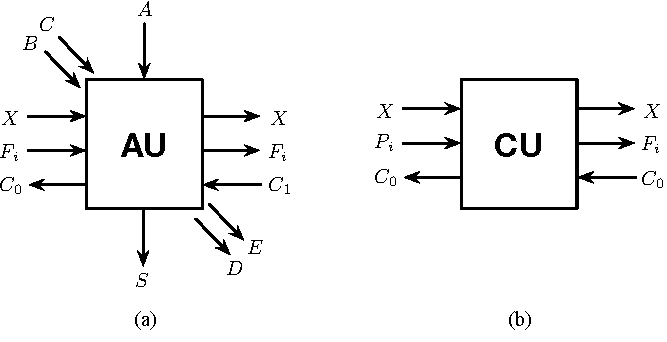
\includegraphics[width=3.0in]{fig/aucu_cells.pdf}\vspace{-3ex}
    \caption{Structure of the basic GPCA cells: (a) arithmetic unit, (b) control unit  (adapted from the figures shown in~\cite{4,2}).} \label{fig:structure}
    \vspace{-3ex}
\end{figure}    

\vspace{-3ex}
\section{Proposed Designs}
We will explain the proposed Boolean expressions for all the output signals of AU first, then the design of CU will be presented.

In terms of the outputs $S$ and $C_0$, from~\eqref{eqs:au} we can see the
subexpression $(B \oplus X)$ is appeared in both expressions. Moreover, the internal node $n_2$ in~\eqref{eqs_maj:au} actually preforms the same operation using MAJ/NOT primitives, i.e., $n_2 = B \oplus X$.
The recent exact synthesis approach~\cite{soeken2017exact} indicates the two- or three-input XOR functions can be realized by at least three MAJ gates. Hence, the expression of $n_2$ in~\eqref{eqs_maj:au} is already optimal in size and depth.
Since the XOR$_3$ gate was proposed in the literature, we make use of MAJ/NOT/XOR$_3$ based expressions for the design.
For the output $C_0$, we replace $n_2$ as $\mathbb{X}(B, X, 0)$, then
\begin{equation}\label{ex_C0}
C_{0} = \mathbb{M}(\mathbb{X}(B, X, 0), A, C_{1})
\end{equation}

For the output $S$, since $(a \oplus b)c + a\bar c = a \oplus bc$ holds, we can assign $a = A$, $b = (B \oplus X) \oplus C_1$, and $c = F_i$. Then
the expression of $S$ in~\eqref{eqs:au} is rewriten as
\begin{subequations}\label{ex_S}
\begin{align}
S &= (((B \oplus X) \oplus C_1)F_i) \oplus A \notag \\
  &= \mathbb{X}(\mathbb{M}(\mathbb{X}(\mathbb{X}(B, X, 0), C_{1}, 0), F_{i}, 0), A, 0) \label{eq:S2} \\
  &= \mathbb{X}(\mathbb{M}(\mathbb{X}(B, X, C_1), F_i, 0), A, 0). \label{eq:S1} 
\end{align}
\end{subequations}
Equation~\eqref{eq:S1} requires only three MAJ/XOR$_3$ operations, in contrast, equation~\eqref{eq:S2} needs one additional XOR$_3$ operation but it can share the node $\mathbb{X}(B, X, 0)$ appeared in~\eqref{ex_C0}.
We reserve both the designs for further evaluations in QCA technology.


%Minimizing the number of wire-crossing in the logic network is of high interest for the QCA technology~\cite{nath2017optimal}.
%For the single-layer restriction, the wire-crossing cannot be implemented.
%Moreover, too many wire-crossings increase the design complexities of a QCA layout since more area and timing are required.

\begin{figure}[b]
\centering
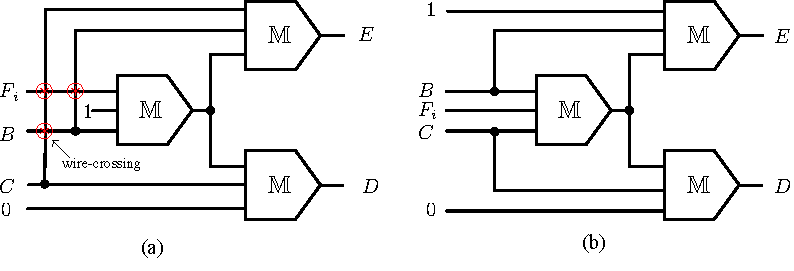
\includegraphics[width=3.5in]{fig/wire_cross.pdf}\vspace{-2ex}
\caption{Two logic networks for the outputs $D$ and $E$, (a) The expressions proposed by GPCA\hspace{-0.2em}~\cite{2} may face wire-crossing problem, (b) Our design.}
\label{fig:wire_cross}
\end{figure}

The outputs of $D$ and $E$ is relatively simple. The logic network proposed in~\cite{2} is shown in Fig.~\ref{fig:wire_cross}(a), in which signals may face the wire-crossing problem. The proposed logic network for outputs $D$ and $E$ is shown in Fig.~\ref{fig:wire_cross}(b), in which the wire-crossing problem is solved.
For the output $D$, the expression is
\begin{equation}\label{eq:D}
D = \mathbb{M}(\mathbb{M}(F_{i}, B, C), C, 0).
\end{equation}
By expansion and simplification, one can verify the function equivalence of~\eqref{eq:D} and the $D$ expression in~\eqref{eqs_maj:au}.
\begin{equation}
\begin{split}
D &= (F_iB + F_iC + BC)C = F_iBC + F_iC + BC \\
  &= F_iC + BC = (F_i + B)C \\
  &= \mathbb{M}(\mathbb{M}(F_i, B, 1), C, 0 )
\end{split}
\end{equation}
Similarly, the output $E$ is represented as
\begin{equation}\label{eq:E}
E = \mathbb{M}(\mathbb{M}(F_{i}, B, C), B, 1)
\end{equation}
such that the subexpression $\mathbb{M}(F_{i}, B, C)$ is shared with~\eqref{eq:D}.


\begin{figure}[t]
\centering
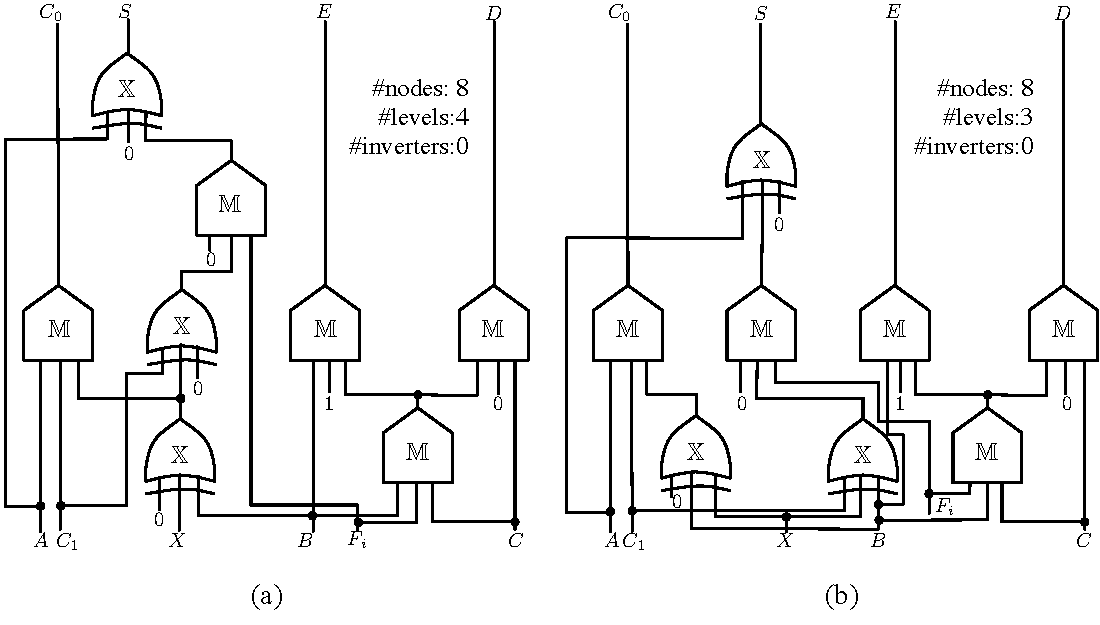
\includegraphics[width=3.5in]{fig/au_netlist.pdf}\vspace{-2ex}
\caption{The logic networks of the proposed design of AU, we make use of (a) \eqref{eq:S2}, (b)~\eqref{eq:S1} as the expression for the output $S$.\vspace{-1ex}}\vspace{-2ex}
\label{fig:au_netlist}
\end{figure}

 \begin{figure}[b]\vspace{-1ex}
     \centering
     \subfigure[]{
             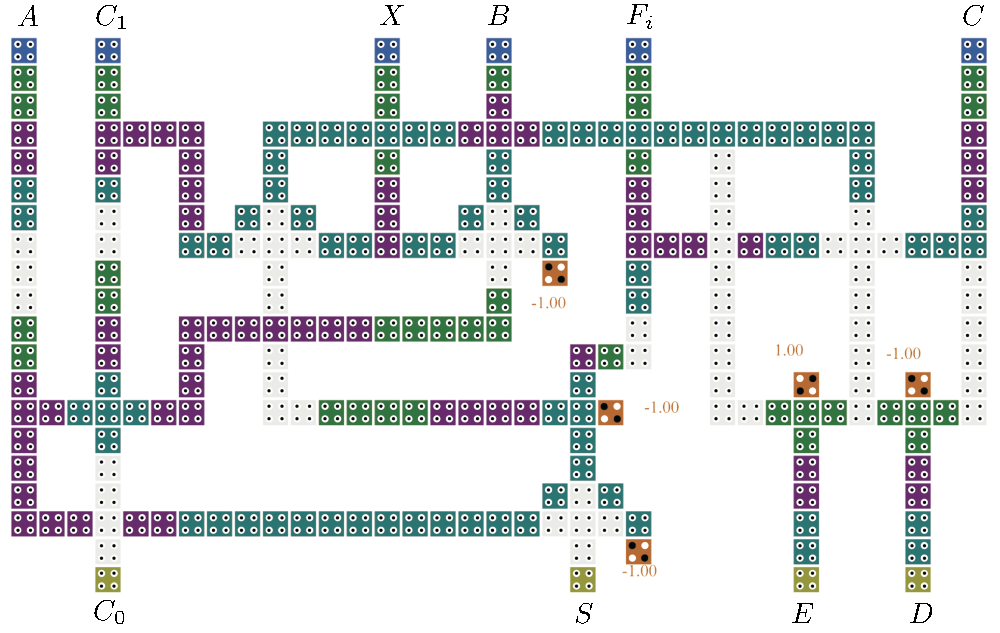
\includegraphics[width=2.3in]{fig/AU_300.pdf}
     }
     \subfigure[]{
            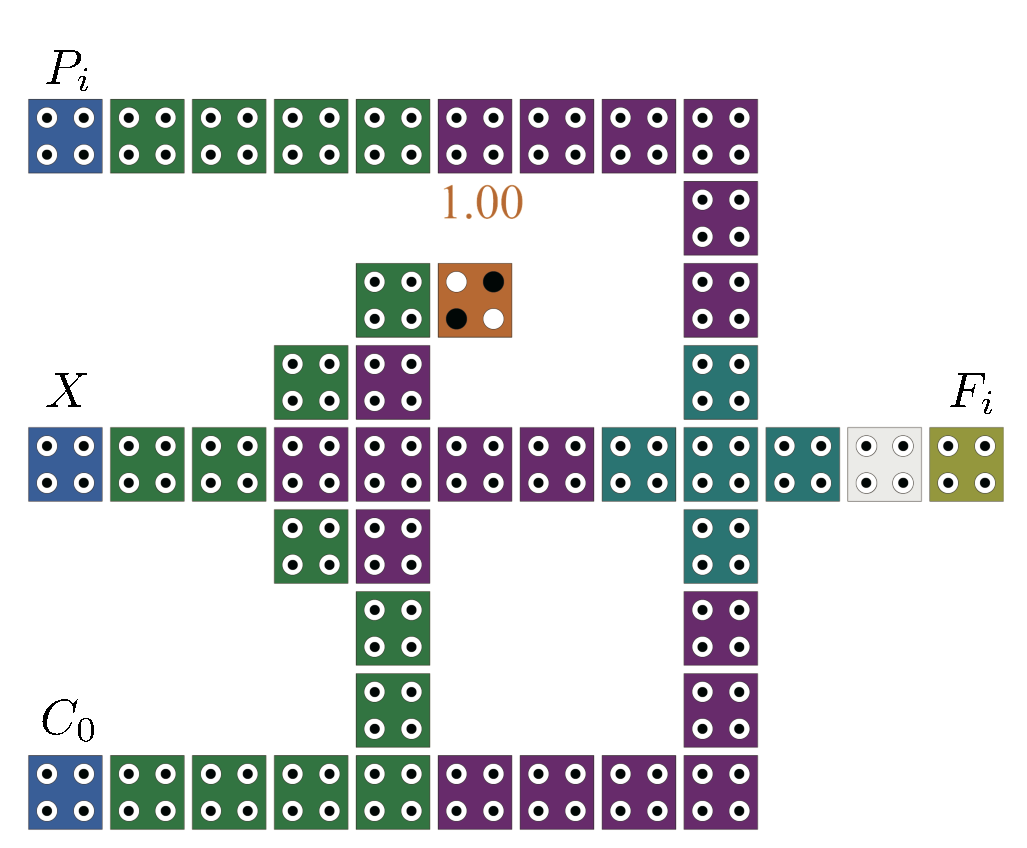
\includegraphics[width=1.0in]{fig/CU_300.pdf}
     }\vspace{-1ex}
     \caption{The single-layer QCA layouts of the proposed (a) AU and (b) CU.}\label{fig:cu_au}
 \end{figure}

The expressions of the AU are the collections of equations~\eqref{ex_C0},~\eqref{ex_S},~\eqref{eq:D}, and~\eqref{eq:E}.
Since~\eqref{ex_S} has two versions of expression, i.e., \eqref{eq:S2} and \eqref{eq:S1}, we present the logic network of both of the two versions in Fig.~\ref{fig:au_netlist}. 
The GPCA cell designs adopt the AU design shown in Fig.\ref{fig:au_netlist} (a) and (b) are named ``\emph{Design A}'' and ``\emph{Design B}'', respectively. 
Both of the AU designs require eight gates, including five MAJ gates and three XOR$_3$ gates. The number of logic levels of Fig.~\ref{fig:au_netlist}(b) is three while the one in Fig.~\ref{fig:au_netlist}(a) is four.
Besides, no inverters are required for both of the designs.
The main difference is the usage of the XOR$_3$ operation. Fig.~\ref{fig:au_netlist}(b) contains one fully-utilized XOR$_3$ node by rewriting $(B \oplus X) \oplus C_1$
into $\mathbb{X}(B, X, C_1)$. Since the node $\mathbb{X}(B, X, 0)$ has two fanouts in Fig.~\ref{fig:au_netlist}(a), we still need this node in~Fig.~\ref{fig:au_netlist}(b) for functional equivalence.
In terms of CU part, the design proposed in~\cite{2} needs three MAJ gates and one inverter. Due to $ab + \bar b c = \mathbb{M}(a, c, \overline{a \oplus b}) = \mathbb{M}(a, c, \mathbb{X}(a,b,1))$, we can assign $a = C_0$, $b = X$, and $c = P_i$. Then the expression of $F_i$ can be rewritten as
\begin{equation}\label{Fi_xmg}
F_{i} = \mathbb{M}(\mathbb{X}(X,C_{0},1),P_{i},C_{0}).
\end{equation}
Note that a constant `1' input in XOR$_3$ gate leads to the inversion of the XOR operation over the other two inputs. Hence, the inverter is also eliminated thanks to the usage of XOR$_3$ operation.

The comparison results of different logic-gate implementations are displayed in Table~\ref{tab:logic}.
By introducing the XOR$_3$ gate, our designs have a fewer number of logic gates/levels, and wire-crossings than previous research, which, in turn, could result in less area/delay, and design complexity of QCA layouts. \emph{Design B} has an advantage on the logic level compared to \emph{Design A} while the number of logic gates is the same.
%In comparison, the design proposed in~\cite{2} requires twelve MAJ gates, six levels, and five inverters. Thus, our design has more compact representations.

\begin{table}[t]
\caption{Comparison Results of the Logic-gate Implementations}\vspace{-2ex}
    \centering
    \begin{tabularx}{\linewidth}{Xccccccccc}
            \toprule
\multirow{2}{*}{Cells}& \multicolumn{3}{c}{Designs in~\cite{2}}&\multicolumn{3}{c}{\emph{Design A}} & \multicolumn{3}{c}{\emph{Design B} }\\
            \cmidrule(lr){2-4} \cmidrule(lr){5-7}\cmidrule(lr){8-10}
            & G & L & C & G & L & C & G & L & C \\
            \midrule
            AU & 17 & 8 & 27 & 8 & 4 & 5 & 8 & 3 & 5\\
            CU & 4 & 3 & 1 & 2 & 2 & 0 & 2 & 2 & 0\\
            \midrule
            Total & 21 & 11 & 28 & 10 & 6 & 5 & 10 & 5 & 5 \\
            \bottomrule
     \end{tabularx}~\label{tab:logic}
         \scriptsize
\begin{flushleft}
G/L/C: the number of logic gates/levels, and wire-crossings.\\
Primitives used in~\cite{2} is MAJ/NOT, while MAJ/NOT/XOR$_3$ in the proposed design.     
\end{flushleft} \vspace{-6ex}
\end{table}

\begin{table}[b] \vspace{-4ex}
\caption{Comparison Results of the AU Designs}\vspace{-2ex}
    \centering
    \begin{tabularx}{\linewidth}{Xccccc}
            \toprule
        AU & Type & Area ($\upmu m^{2}$)& Latency & Cells count \\
        \midrule
        \emph{Design A} & Multi-layer & 0.25      & 1.5            & 238                          \\
        \midrule
        \multirow{2}{*}{\emph{Design B}} & Multi-layer & 0.21      & 1              & 217                           \\
        & Single-layer & 0.31 & 2 & 245 \\
        \bottomrule
    \end{tabularx}
    \label{tab:au}
\end{table}\vspace{-2ex}

%\begin{figure*}[t]
%    \centering
%    \includegraphics[height=12cm]{fig/pipeline_array.jpg}
%    \caption{ The QCA layout of our proposed array}
%\end{figure*}
%%%%%%%%%%%%%%%%%%%%%%%%%%%%%%%%%%%%%%%%%%%%%%%%%%%%%%%%%%%%%%%%%%%%%%%
\begin{table*}[h]
\caption{Comparison Results of the Proposed GPCA versus the Designs Presented in~\cite{2}}\vspace{-3ex}
\centering
\begin{tabularx}{\textwidth}{Xrrrrrrrrr}
\toprule
            \multirow{2}{*}{Designs}& \multicolumn{3}{c}{GPCA~\cite{2}}&\multicolumn{6}{c}{ Ours }\\
            \cmidrule(lr){2-4} \cmidrule(lr){5-10}
            &Area ($\mu m^2$) & Latency & Cells count &Area ($\mu m^2$) & \% &Latency & \% & Cells count &\% \\
            \midrule
            AU &0.68 &4 &682 &0.21 &69.12 &1 &75.00 &217 &68.18 \\
            CU & 0.11&1.5&77&0.05&54.55&1&33.33&44&42.86\\
            GPCA (n=3)&23.35&34&15098&17.06&26.94&25&26.47&10312&31.70\\
            GPCA (n=4)&39.44&51&26698&29.80&24.44&39&23.53&17258&35.36\\
            GPCA (n=5)&59.47&71&42174&46.80&21.30&56&21.13&26094&38.13\\
            \midrule
            Average improvement&  &  & & & 39.27\% & &35.89\% && 43.25\% \\
            \bottomrule
\end{tabularx}~\label{tab:result}\vspace{-3ex}
\end{table*}
%%%%%%%%%%%%%%%%%%%%%%%%%%%%%%%%%%%%%%%%%%%%%%%%%%%%%%%%%%%%%%%%%%%%%%%


\begin{figure*}[h]
    \centering \scriptsize
    \subfigure[]{
        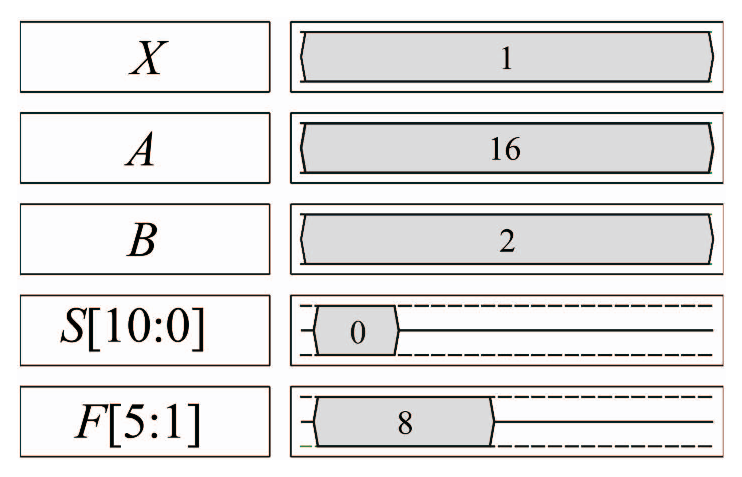
\includegraphics[width=1.5in]{fig/division.eps}\label{div}
    }\hfil
    \subfigure[]{
        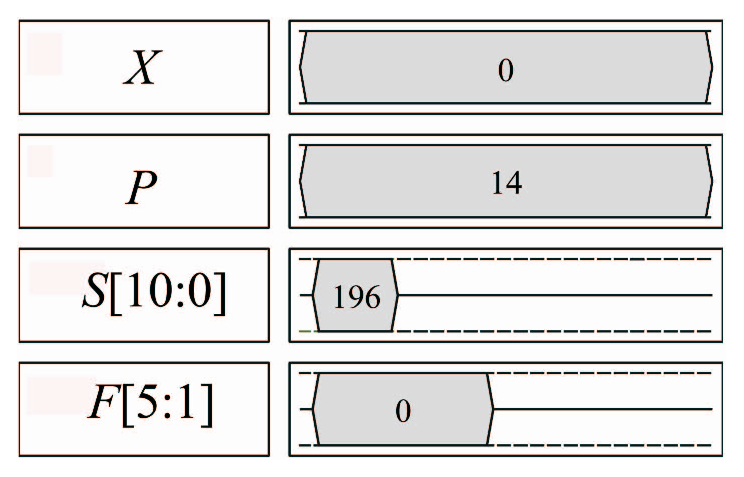
\includegraphics[width=1.5in]{fig/squaring.eps}\label{square}
    }\hfil
    \subfigure[]{
            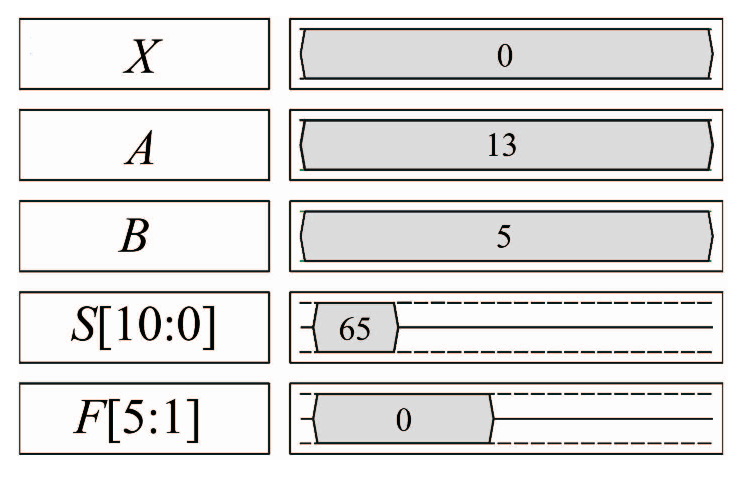
\includegraphics[width=1.5in]{fig/multiplication.eps}\label{multiplier}
    }\hfil
    \subfigure[]{
          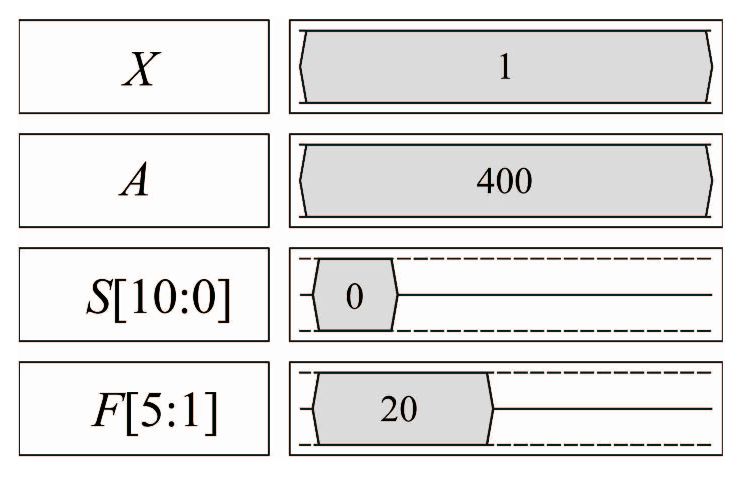
\includegraphics[width=1.5in]{fig/square_rooting.eps}\label{square_rooting}
    }\vspace{-2ex}
    \caption{Simulation results for (a) Division, (b)Squaring, (c) Multiplication, and (d)Square rooting.}\label{tt_array} \vspace{-3ex}
\end{figure*}

\vspace{-1ex}
\section{Experimental Results and Comparison}\vspace{-1ex}
In this section, the simulation results of our designs were presented.
All the designs and simulations are implemented by QCADesigner 2.0.3.
We have set the same parameters with the ones presented in~\cite{2}.
The XOR$_3$ gate proposed in~\cite{3} is adopted in our designs.
And the clock-zone based wire-crossing technique~\cite{shin2013wire} is used for single-layer QCA design.
The latency of the design is represented by the number of required operation clock cycles.

\textbf{AU Designs:}
We realized the proposed AU design in both single- and multi-layer design methods.
The single-layer one is more practical for QCA fabrication. 
But for fair comparison and evaluation with the state-of-the-art, the multi-layer approach is also established.
The comparison results of AU designs are shown in Table~\ref{tab:au}, which indicate our multi-layer realization of  \emph{Design B} has a better performance in both the area and delay. 
Therefore, we adopt \emph{Design B} as the building block for the subsequent $n$-bit GPCA designs.
The single-layer QCA layouts of our proposed AU and CU are shown in Fig.~\ref{fig:cu_au}(a) and (b), respectively, thanks to our reduced number of wire-crossings. Note that CU design has no wire-crossing, thus the layout of CU is naturally in single-layer. 
%Fig.~\ref{fig:cu_au} shows the QCA layout of our proposed AU and CU, from which we can see that both of the AU and CU have the same delay of 1 clock cycle.

\textbf{Comparisons with the State-of-the-Art:}
The proposed AU and CU are the building blocks to construct the GPCA for performing arithmetic operations of any number of bits.
Comparison results of the proposed designs with the state-of-the-art approach~\cite{2} is given in Table~\ref{tab:result}.
It can be seen from the table that both the AU and CU designs achieve better performance in the area, latency, and cells count.
The proposed AU design has reduced the area by 69.12\% from 0.68 $\mu m^2$ to 0.21 $\mu m^2$ and the latency is reduced by 75\% from 4 clock cycles to 1 clock cycle. Moreover, the cells count is reduced from 682 to 217, which is 68.18\% improvement. The better performance can be also seen for the CU design.    
This advantage also carries over into the $n$-bit GPCA designs. As an example, the proposed 5-bit pipeline array design has a total number of 26,094 QCA cells and an area of 46.80 $\mu m^2$ with a latency of 56 clock cycles, while the one presented in~\cite{2} has a total number of 42,174 QCA cells and an area of 59.47 $\mu m^2$ with a latency of 71 clock cycles. On average, the proposed design has reduced the area, latency, and cells count by 39.27\%, 35.89\%, and 43.25\%, respectively.  

The proposed AU and CU designs reduced the clock cycles by 3 and 0.5 compared with GPCA in~\cite{2}, respectively. Thus, theoretically speaking, the delay of each level in GPCA can be reduced by 3.5 clock cycles. However, in favor of the clock design of the QCA layout, we added a 0.5 clock cycle per level in our design. 
As a result, the delay of the first level has 6 clock cycles and the calculation formula of the delay is as given in~\eqref{delay}. The reader can refer to~\cite{2} for details of delay calculation.
\begin{equation}\label{delay}\vspace{-1ex}
\begin{split}
& Delay =1 + \sum\limits_{i=1}^{n}(5  + 3(i-1))\\
\end{split}\vspace{-1ex}
\end{equation}
Generally, for the $n$-bit GPCA design, the proposed design can reduce $3n$ clock cycles compared with the GPCA presented in~\cite{2}.
For example, the latency of the 5-bit GPCA is $Delay_{n=5}=56$, in which $3n=3 \times 5=15$ clock cycles are saved. 

Fig.~\ref{tt_array} shows the simulation result of our GPCA. The input `$X$' is a control line, which made logical zero or one for different arithmetic computations.
For division, we set $A$'s as (10000)$_2$ (binary number, 16 in decimal) and $B$'s as (10)$_2$ we got the result of (1000)$_2$ in $F$'s and the remainder of 0 in $S$'s as show in~Fig.~\ref{div}. In Fig.~\ref{square}, we set $P$'s as (1110)$_2$ and we got the result of (11000100)$_2$ in $S$'s for squaring operation. For multiplication in Fig.~\ref{multiplier}, we set $A$'s (1101)$_2$ and $B$'s as (101)$_2$ and we got the result of (1000001)$_2$ in $S$'s. For square rooting in Fig.~\ref{square_rooting}, we put $A$'s as (110010000)$_2$ and we got the result of (10100)$_2$ in $F$'s and the remainder of $0$ in $S$'s.

\vspace{-2ex}
\section{Conclusions}
In this letter, we proposed a QCA design for generalized pipeline cellular array (GPCA). 
Unlike existing GPCA design using only the majority logic network, the proposed array is constructed by additionally introducing three-input XOR (XOR$_3$) gates. Thus, the GPCA is represented by a hybrid logic network by using majority, inverter, and XOR$_3$ primitives. The proposed arithmetic and control unit have a significant reduction of area, latency, and cells count. On average, we can achieve 39.27\%, 35.89\%, 43.25\% reduction of area, delay and cells count compared with the state-of-the-art.

\vspace{-2ex}
\ifCLASSOPTIONcompsoc
  \section*{Acknowledgments}
\else
  \section*{Acknowledgment}
\fi
This work was supported in part by NSFC under Grant No 61871242 and in part by K.C.Wong Magna Fund in Ningbo University.
\vspace{-2ex}
\ifCLASSOPTIONcaptionsoff
  \newpage
\fi
\tiny
\bibliographystyle{IEEEtranS}
\bibliography{./IEEEabrv,./refs}

\begin{appendices} 
	\setlength{\parindent}{0pt}
	\setlength{\parskip}{2em}
\section{AUTHORS’ RESPONSE TO REVIEWERS} 
\normalsize
We first thank the Editors and Reviewers for conducting the peer-review of our manuscript. In the revised version, we have adequately addressed the reviewers’ comments.
The provided comments have helped to improve the technical contents as well as the presentation of our work. 
%All changes with respect to the original submission have been highlighted in red in the revised manuscript. 


\subsection{Reviewer 1}
{\bfseries Comment-1: The author should clearly explain how they have come up with the design given in Figure 5. Figure 5 is not mentioned in the text at all.}

{\bfseries Response:} Thanks for your suggestion. Since GPCA can perform the operations of any number of bits, the high-performance AU and CU designs lead to cumulative improvement for $n$-bit GPCA design. 
Figure 5 (in the submitted version) is the 5-bit GPCA whose computer structure is originally demonstrated in~\cite{4}. 
We add description in Section 1.
As Reviewer 3 suggested, we have removed Figure 5 and added more technical details to make the contribution clearer.

%With the proposed QCA designs of the basic GPCA cell, the AU and CU are then used as the building blocks of this 5-bit GPCA. 
%Figure 5 is used to display the QCA layout and clock distributions of our proposed GPCA, which can be verified by the QCADesigner tool. But we failed to add some description about it in the submitted manuscript.
%The logic structure of $5$-bit GPCA whose QCA layout is shown in Figure 5 has been proposed in~\cite{4}, we just need to use proposed basic GPCA cell to form it.


{\bfseries Comment-2: Equations 1, 3 and others are given in reference 9. I fail to understand why authors do not describe their papers by building on reference 9 rather than building on reference 8.}

{\bfseries Response:} Thanks for your kind suggestion. The Boolean expressions of GPCA are firstly proposed by reference [8] (reference~\cite{4} in the revised version), which are based on two-input XOR/AND/OR and single-input NOT operations. In fact, designs of [9] (reference~\cite{2} in the revised version) and ours are both based on the Boolean expressions presented in [8]. 

{\bfseries Comment-3: The authors should start their papers by giving a review of reference 9 and then illustrate and prove how they have made modifications in reference 9.}

{\bfseries Response:} We have added Section 2 for related work and given a review of [9] (reference~\cite{2} in revised vision) in Section 3. The proposed design is discussed in Section 4.

\subsection{ Reviewer 2}
{\bfseries Comment-1: Although the topic looks interesting, I am not sure how much contribution this paper adds to the state-of-the-art. In other words, the paper came up with different hardware implementation for the work proposed in reference [9].}

{\bfseries Response:} Thanks for the comments. Indeed, we proposed a logic representation over the gate basis \{MAJ, NOT, XOR$_3$\} of the basic GPCA cell. We implemented the proposed design using QCA technology for a fair comparison with the work presented in reference [9] (reference~\cite{2} in revised vision). 
However, it can be implemented using other technologies once the primitives in new technology are ready for fabrication.
For example, the two-dimensional polarity-controllable transistors can realize logic gates \{MAJ, NOT, XOR$_3$\} with fewer transistors than conventional CMOS logic~\cite{resta2018doping}.    

{\bfseries Comment-2: As the authors mentioned the new hardware implementation resulted in higher area efficiency and lower latency. If QCA is the way the future technology is going to go, we need more innovations to push this technology into the market. }

{\bfseries Response:} Thanks for the concerns. We agree that QCA is still an emerging technology. The proposed QCA design is used for comparison and validation. Other techniques that in favor of \{MAJ, NOT, XOR$_3$\} realizations can also get benefits from the proposed design.
%
%Thanks for your kind suggestion. Firstly, we have added a discuss of the importance of wire-crossing problem in the second paragraph of Section 3.1 and some details have been discussed in Section 4. Wire-crossing may lead to many difficulties, including crosstalk and additional power dissipation. Thus, we should reduce wire-crossing when we implement a circuit in QCA as many as possible. From TABLE 1 we can see that just for the AU and CU part, our design reduces the number of wire-crossing from 28 of reference [9] (Reference~\cite{2} in revised vision) to only 5 which has a great improvement. In addition, we have added another single-layer design of AU based on clock-zone approach to make our paper more convincing in Section 5.1.

{\bfseries Comment-3: The paper lacks architectural innovation. I believe the proposed method needs to be combined with some innovation in the hardware to show the actual benefit. The reported improvements are coming from the gate-level implementation, rather than architecture.}

{\bfseries Response:} Thanks for the comments. We do not address the architecture design issue directly. But we believe logic design and implementation are also playing essential roles in modern computer architecture designs.
We rewrite Section 1 to give a more explicit description of our work, and lots of technical details, comparisons, and evaluations are added in the revised version.
For the QCA design itself, from the perspective of fabrication, we also established a single-layer QCA layout. More details can be found in Section 5.  
Thanks again.  

\subsection{ Reviewer 3}
{\bfseries Comment-1: It would be nice to better highlight the downsides of prior work. I felt section 2.1 ended abruptly without describing the issues with these gate counts.}

{\bfseries Response:} Thanks for your kind suggestion. We have added the downsides of prior work in Section 3 in detail. It can be found that only four MAJ gates in prior work are fully utilized (i.e., with no constant inputs), the remaining eleven MAJ gates are partially utilized (i.e., with one constant input). Further improvement can be achieved if we make better use of MAJ gates or introducing new XOR$_3$ primitive.

{\bfseries Comment-2: brief discussion/overview of the wire-crossing problem would be nice. I understand at a very high level from VLSI that wire-crossings are difficult but are they *more* difficult for QCA design and layout? If so, briefly explain why and give a sense for how painful it is. That will help readers understand how important your contribution is. }

{\bfseries Response: } Thanks for your kind suggestion. We have added a brief introduction to the wire-crossing problem in the third paragraph of Section 3. Wire-crossing may lead to many difficulties, including crosstalk and additional power dissipation. Moreover, the wire-crossing increase the QCA design complexity. 

{\bfseries Comment-3: It is difficult in text to understand the trade-offs between different design choices. For example, following all of the changes in various gate counts of page 2 is tedious for the reader. Putting these numbers into a table or using relative numbers when comparing all design choices of each expression would be helpful. }

{\bfseries Response:} Thanks for your kind suggestion. We have added Table 1 to show the comparisons of all designs, and the results are analyzed in the last paragraph of Section 4.

{\bfseries Comment-4: It would also be nice to have some sort of progressive information to show a “path” to your final design through the various design points you evaluated.}

{\bfseries Response:} Thanks for your kind suggestion. We have revised the paper in a specific order according to your suggestions. Now it may become easier to understand the progressive information to our final design.

{\bfseries Comment-5: There is plenty of white space and text for you to compress to add more to the paper. For example. The right column of the first page is very sparse, and the text below section 2 could be completely deleted if that space is useful to add more figures or explanatory text. X }

{\bfseries Response:} Thanks for your valuable comments. We have added more details to our paper and have filled the white space.

{\bfseries Comment-6: Figure 5 is very large and for me did not add much value to the paper. Is it to show that there are few wire crossings? Is there any way to shrink it without making it unreadable? Or maybe consider removing it? (although it is a pretty figure!) }

{\bfseries Response:} Thanks for your kind suggestion. We have deleted Figure 5, and more details have been added to make the paper more accessible and clearer to understand.

{\bfseries Comment-7: Instead of using a citation as a noun (i.e. “We compare against [9]” or “[9] used 4 gates”) you should really use the proper name for the technique and then cite it. I think GPCA[9] would be clearer. This makes Table 1 especially difficult to parse on first read.}

\noindent {\bfseries Response: } Thanks for your kind suggestion. We have addressed the issue in the revised version.
\end{appendices} 

\end{document}


